The PDF, CDF of each $X_{1},X_{2},X_{3},\dots$ is 
\begin{align}
\tag{72.1}
    f_{X_{i}}(x)=\begin{cases}
	1, & 0< x<1 \\~\\[-1em]
	0, & otherwise
	\end{cases} 
\end{align}
\begin{align}
\tag{72.2}
	F_{X_{i}}(x)=\begin{cases}
	x, & 0< x<1 \\~\\[-1em]
	1, & x\geq 1\\~\\[-1em]
	0, & otherwise
	\end{cases} 
\end{align}
$\forall i\in \mathbb{N}$.
Then, as $T_{n}=max\{ X_{1},X_{2},\dots,X_{n}\}$,
\begin{align}
\tag{72.3}
    f_{T_{n}}(x)=\begin{cases}
	nx^{n-1}, & 0< x<1 \\~\\[-1em]
	0, & otherwise
	\end{cases} \\
\tag{72.4}
	F_{T_{n}}(x)=\begin{cases}
	x^{n}, & 0< x<1 \\~\\[-1em]
	1, & x\geq 1\\~\\[-1em]
	0, & otherwise
	\end{cases} 
\end{align}
NOTE : If $Y=aX+b$ and $a<0$, then
\begin{align}
\tag{72.5}
\label{june/2013/72/eq:form}
    F_{Y}(y)=1-F_{X}\brak{\dfrac{y-b}{a}}
\end{align}
\begin{enumerate}
\item OPTION-1:\\
Convergence in Probability :\\
A sequence of random variables $X_{1},X_{2},X_{3},\dots$ converges in probability to a random variable $X$, shown by $X_{n}\xrightarrow[]{p}X$, if
\begin{align}
\tag{72.6}
    \displaystyle\lim_{n\to\infty}\pr{|X_{n}-X|\geq\epsilon}=0,\forall\epsilon>0
\end{align}
To evaluate : $\displaystyle\lim_{n\to\infty}\pr{|T_{n}-1|\geq\epsilon},\forall\epsilon>0$
\begin{align}
\tag{72.7}
    &\displaystyle\lim_{n\to\infty}\pr{|T_{n}-1|\geq\epsilon}=\displaystyle\lim_{n\to\infty}\pr{1-T_{n}\geq\epsilon}\\
\tag{72.8}
    &=\displaystyle\lim_{n\to\infty}\pr{T_{n}\leq1-\epsilon}=\displaystyle\lim_{n\to\infty}F_{T_{n}}(1-\epsilon)
\end{align}
\begin{align}
\tag{72.9}
    F_{T_{n}}(1-\epsilon)=\begin{cases}
	(1-\epsilon)^{n}, & 0< \epsilon<1 \\~\\[-1em]
	0, & \epsilon\geq 1
	\end{cases}
\end{align}
\begin{align}
\tag{72.10}
    \because\displaystyle\lim_{n\to\infty}(1-\epsilon)^{n}=0 \text{ for } 0< \epsilon<1\\
    \tag{72.11}
    \therefore \displaystyle\lim_{n\to\infty}\pr{|T_{n}-1|\geq\epsilon}=0,\forall\epsilon>0
\end{align}
$\therefore T_{n}$ converges to 1 in probability.
\item OPTION-2:\\
Convergence in Distribution :\\
A sequence of random variables $X_{1},X_{2},X_{3},\dots$ converges in distribution to a random variable $X$, shown by $X_{n}\xrightarrow[]{d}X$, if
\begin{align}
\tag{72.12}
    \displaystyle\lim_{n\to\infty}F_{X_{n}}(x)=F_{X}(x)
\end{align}
for all $x$ at which $F_{X}(x)$ is continuous.\\
To evaluate : $\displaystyle\lim_{n\to\infty}F_{n(1-T_{n})}(x)$\\ 
Substituting $a=-n,b=n$ in \eqref{june/2013/72/eq:form},
\begin{align}
\tag{72.13}
    F_{n(1-T_{n})}(x)=1-F_{T_{n}}\brak{1-\dfrac{x}{n}}
\end{align}
\begin{align}
\tag{72.14}
    F_{T_{n}}\brak{1-\dfrac{x}{n}}=\begin{cases}
	\brak{1-\dfrac{x}{n}}^{n}, & 0< x<n \\~\\[-1em]
	1, & x\leq 0\\~\\[-1em]
	0, & x\geq n
	\end{cases} 
\end{align}
\begin{align}
\tag{72.15}
    \because\displaystyle\lim_{n\to\infty}\brak{1-\dfrac{y}{n}}^{n}=e^{-y}
\end{align}
\begin{align}
\tag{72.16}
\label{june/2013/72/eq:bcdf}
    \therefore\displaystyle\lim_{n\to\infty} F_{T_{n}}\brak{1-\dfrac{x}{n}}=\begin{cases}
	e^{-x}, & 0< x<n \\~\\[-1em]
	1, & x\leq 0\\~\\[-1em]
	0, & x\geq n
	\end{cases} 
\end{align}
\begin{align}
\tag{72.17}
\label{june/2013/72/eq:cdf}
    \therefore F_{n(1-T_{n})}(x)=\begin{cases}
	1-e^{-x}, & 0< x<n \\~\\[-1em]
	0, & x\leq 0\\~\\[-1em]
	1, & x\geq n
	\end{cases} 
\end{align}
\begin{figure}[h!]
\centering
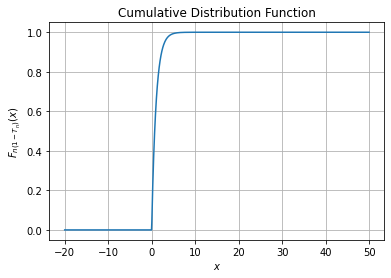
\includegraphics[width=\columnwidth]{solutions/2013/june/72/figures/Assignment9}
\caption{CDF}
\label{june/2013/72/plot}
\end{figure}
$\therefore n(1-T_{n})$ converges in distribution to a random variable with CDF in \eqref{june/2013/72/eq:cdf}.
\item OPTION-3:\\
Convergence in Distribution :\\
A sequence of random variables $X_{1},X_{2},X_{3},\dots$ converges in distribution to a random variable $X$, shown by $X_{n}\xrightarrow[]{d}X$, if
\begin{align}
\tag{72.18}
    \displaystyle\lim_{n\to\infty}F_{X_{n}}(x)=F_{X}(x)
\end{align}
for all $x$ at which $F_{X}(x)$ is continuous.\\
To evaluate : $\displaystyle\lim_{n\to\infty}F_{n^{2}(1-T_{n})}(x)$\\ 
Substituting $a=-n^{2},b=n^{2}$ in \eqref{june/2013/72/eq:form},
\begin{align}
\tag{72.19}
    F_{n^{2}(1-T_{n})}(x)=1-F_{T_{n}}\brak{1-\dfrac{x}{n^{2}}}
\end{align}
\begin{align}
\tag{72.20}
    F_{T_{n}}\brak{1-\dfrac{x}{n^{2}}}=\begin{cases}
	\brak{1-\dfrac{x}{n^{2}}}^{n}, & 0< x<n^{2} \\~\\[-1em]
	1, & x\leq 0\\~\\[-1em]
	0, & x\geq n^{2}
	\end{cases} 
\end{align}
\begin{align}
\tag{72.21}
    \because\displaystyle\lim_{n\to\infty}\brak{1-\dfrac{y}{n^{2}}}^{n}\text{ is not defined}
\end{align}
$\therefore n^{2}(1-T_{n})$ does not converge in distribution.
\item OPTION-4:\\
Convergence in Probability :\\
A sequence of random variables $X_{1},X_{2},X_{3},\dots$ converges in probability to a random variable $X$, shown by $X_{n}\xrightarrow[]{p}X$, if
\begin{align}
\tag{72.22}
    \displaystyle\lim_{n\to\infty}\pr{|X_{n}-X|\geq\epsilon}=0,\forall\epsilon>0
\end{align}
To evaluate :\\ $\displaystyle\lim_{n\to\infty}\pr{|\sqrt{n}(1-T_{n})-0|\geq\epsilon},\forall\epsilon>0$
\begin{align}
\tag{72.23}
    =\displaystyle\lim_{n\to\infty}\pr{1-T_{n}\geq\dfrac{\epsilon}{\sqrt{n}}}\\
\tag{72.24}
    =\displaystyle\lim_{n\to\infty}\pr{T_{n}\leq1-\dfrac{\epsilon}{\sqrt{n}}}\\
\tag{72.25}
    =\displaystyle\lim_{n\to\infty}F_{T_{n}}\brak{ 1-\dfrac{\epsilon}{\sqrt{n}}}
\end{align}
\begin{align}
\tag{72.26}
    F_{T_{n}}\brak{1-\dfrac{\epsilon}{\sqrt{n}}}=\begin{cases}
	\brak{1-\dfrac{\epsilon}{\sqrt{n}}}^{n}, & 0< \epsilon< \sqrt{n}\\~\\[-1em]
	0, & \epsilon\geq \sqrt{n}
	\end{cases}
\end{align}
\begin{align}
\tag{72.27}
    \because\displaystyle\lim_{n\to\infty}\brak{1-\dfrac{\epsilon}{\sqrt{n}}}^{n}=0 \text{ for } 0< \epsilon<\sqrt{n}\\
    \tag{72.28}
    \therefore \displaystyle\lim_{n\to\infty}\pr{|\sqrt{n}(1-T_{n})-0|\geq\epsilon}=0,\forall\epsilon>0
\end{align}
$\therefore\sqrt{n}(1-T_{n})$ converges to 0 in probability.
\end{enumerate}
\begin{lstlisting}
Hence, options 1), 2), 4) are correct.
\end{lstlisting}